% Use only LaTeX2e, calling the article.cls class and 12-point type.
\documentclass[12pt]{article}
\usepackage{amsmath} 
\usepackage{amssymb}
\numberwithin{table}{section}
\numberwithin{figure}{section}
\usepackage{floatrow}
\usepackage{longtable}
\usepackage{graphicx}
\usepackage[
    %backend=biber, 
    natbib=true,
    style=numeric,
    sorting=none
]{biblatex}
\usepackage{booktabs}
\usepackage{tabularx}
\usepackage[export]{adjustbox}
\addbibresource{references.bib}
\allowdisplaybreaks

\newcommand{\R}{\mathbb{R}}

\usepackage[letterpaper, margin=1.5cm]{geometry}
% The following parameters seem to provide a reasonable page setup.

% \topmargin 0.0cm
% \oddsidemargin 0.0cm
% \textwidth 16cm 
% \textheight 20cm
% \footskip 3.0cm

% Include your paper's title here
\title{\vspace{-2.5em}AI Tetris - A CS3243 Project (Group 21)}
\author{Lau Kar Rui (A0155936U), Tan Chee Wee (A0155400W), 
\\Poh Jie (A0158523A), Matilda (A0178867A)}
\date{}


% Start of document.
\begin{document} 
% 1.5 space the manuscript.
\baselineskip15.0pt
% paragraph spacing
\setlength{\parskip}{0.3em}
\linespread{1.0}
% Make the title.
\maketitle 

\section{Introduction}

We create an utility-based Tetris-playing AI agent with utility weights derived through \emph{Particle Swarm Optimization} (PSO) to maximise the number of cleared rows in a game of Tetris. 

% if got space we explain what tetris is
	
\section{Utility Function}\label{eq:util-fx}
With every new piece, the agent determines the best possible state derivable from the piece and plays it, by simulating all possible states $s_i$ of the board the piece legally can reach (via its orientations and positions). The best state will have the highest utility function value $F(s)$, defined as
	$$F(s) = \sum_{i = 1}^{n} w_if_i(s),$$
with each feature $f_i \in Features$ mapped to a weight $w_i$, where $i = 1...n$, $n$ = number of features. Each $f_i$ derives a real value from a game state. 

\section{Features Used} \label{sec:features}
Table \ref{tab:features} describes the features $f_i$ used to calculate $w_i \in Weights$ when training the agent with the PSO algorithm described in Section \ref{sec:PSO}. 

\begin{longtable}[c]{|p{4cm}|p{12.5cm}|}
\hline
\textbf{Feature}  & \textbf{Description} \\ \hline
\textbf{RowsCleared }      & Number of rows cleared \\ \hline
\textbf{MaxHeightIncrease} & Maximum height increase among all columns \\ \hline
\textbf{AvgHeightIncrease} & Average height increase among all columns \\ \hline
\textbf{AbsoluteDiff}      & Absolute height difference between all columns \\ \hline
\textbf{NumHoles}          & Number of holes; a hole is defined as an empty cell with a non-empty cell above it \\ \hline
\textbf{ColumnTransition}  & Number of column transitions; defined as empty cells adjacent to filled cells in the same column or vice versa \\ \hline
\textbf{RowTransition}     & Number of row transitions; defined as empty cells adjacent to filled cells on the same row or vice versa \\ \hline
\textbf{WellSum}           & Number of empty cells above each columns' top heights which are adjacent to filled cells on both sides \\ \hline
\caption{Features used}
\label{tab:features}
\end{longtable}

\section{Implementation}
% $F$ is applied on every possible next state $s_i$ using the \texttt{StateCopy} mechanism described in Section \ref{sec:statecopy}, and the state with the greatest value is chosen as the new current state.
% * <matilds@live.se> 2018-04-17T04:39:06.452Z:
% 
% not necessary to describe what a state is, we've already brought up state earlier. but also we don't specifically say what weights and features are (I feel like no need)
% 
% ^.

% \subsection{StateCopy} \label{sec:statecopy}
% A \texttt{StateCopy} class was created as an extension of the original \texttt{State} class, serving as a state to apply $F$ on in order to derive the greatest feature value, allowing us to play moves without affecting the original state of the game.

\subsection{Particle Swarm Optimization (PSO)} \label{sec:PSO}
The PSO method is used with a population (a.k.a. swarm) of candidate solutions (a.k.a. particles), which in the search-space of $F$ moves to find the best possible positions (a.k.a. $w_i \in Weights$) for $F(s)$.

The movement of each particle $\vec{x}$ is governed by the \emph{velocity} $\vec{v}$, which is derived from each particle $\vec{x}$'s \emph{personal best position} $\vec{p}$, and the \emph{swarm's best position} $\vec{g}$ through the formulae below, where $\omega$ refers to the inertia, $\phi_p, \phi_g$ the social and cognitive parameter, and $r_p, r_g$ two random values $\in [0...1]$
% think still should put this formula down, then appendix elaborate
\begin{gather*}
\vec{v}\leftarrow \omega\vec{v} + \phi_p r_p ( \vec{p} - \vec{x} ) + \phi_g r_g ( \vec{g} - \vec{x} )
\\
\vec{x}\leftarrow \vec{x} + \vec{v}
\end{gather*}

An \emph{inertia} $\omega$ of lower magnitude allows the swarm to converge faster to a solution (optimality not guaranteed) while the opposite encourages exploring the search-space. The \emph{velocity} of each particle is re-calculated after every iteration (where the Tetris game is played with $\vec{x}$ being the weights of the features) and serves as the swarm's willingness to move in the search-space.

Values for the constants (swarm size $N, \omega, \phi_p, \phi_g$) were first chosen based on values stated in \cite{VanDenBergh2006ATrajectories} and later optimized with the Meta Optimization algorithm discussed in Section \ref{sec:meta-opt}. Details of full algorithm is further elaborated on in Appendix \ref{app:pso}.

% Karrui comments:
% Some misconceptions here: the v-bar equation is basically:
% velocity = inertia * previous velocity + cognitiveConstant*randomValue*(personalbestposition - currentposition) +
% social constant*randomValue*(swarmbestposition - currentposition)
% So this is more than 2 factors velocity and inertia, but many constant parameters, inertia, social+cognitive constant and the variables personalbestposition and swarmbestposition
% This is also why PJ tried to do metaoptimization to see if there are better constant parameters than the one i chose because of another paper.

\subsection{Meta Optimization of PSO}\label{sec:meta-opt}
While literature exists on finding the ideal parameters of PSO \cite{Shi1998ParameterOptimization}, these parameters generally do not have a specific problem in mind. Hence, we wanted to investigate if there exist better parameters for our TetrisAI problem. We turn to the Local Unimodal Sampling (LUS) algorithm \cite{ErikLocalSampling} and its use in the Meta Optimization (MO) Problem \cite{Pedersen2010SimplifyingOptimization}. 

Details of the LUS algorithm can be found in Appendix \ref{app:lus}, but a brief of our usage of it is as follows: random values are generated for the 4 constant parameters (swarm size $N$, inertia $\omega$, cognitive $\phi_p$ and social parameters $\phi_g$). The PSO is then run using these parameters for 100 iterations. If the fitness value of PSO using this set of parameters is better than the best fitness value obtained so far, we do not reduce the search range for the parameters; else we do. In either, new parameters are generated.

The algorithm ran for 10 iterations, each iteration consisting of 100 PSO iterations. The best weights obtained so far was used as the best score seemed to be stuck at around 1 million rows cleared using only the PSO algorithm to see if we could get better results using other parameters.

The 5 best sets of parameters (details available in Appendix \ref{fig:parameters-info}) derived from LUS were compared with 5 sets of the parameters from \cite{VanDenBergh2006ATrajectories} by running 10 sets of PSO, for up to 300 iterations, and comparing the performance of the LUS parameters against the set of parameters from \cite{VanDenBergh2006ATrajectories}. Each run of PSO started with no learned weights. The parameters attained from MO are referred to as \emph{MO1, MO2}, etc, in the order they are displayed in Appendix \ref{fig:parameters-info}. Similarly, the parameters suggested in \cite{VanDenBergh2006ATrajectories} are referred to as \emph{Suggested}.

To reduce the impact of outliers skewing the data, the mean of  the performance of \emph{Suggested} was calculated  for every 50 iterations. The performance of the PSO run was also recorded using MO parameters for every 50 iterations.

\begin{table}[H]
\small
\centering
\caption{Rows cleared every 50 iterations}
\label{tab:compareParameters}
\begin{tabular}{|l|l|l|l|l|l|l|l|}
\hline
\textbf{}              & \textbf{1} & \textbf{50} & \textbf{100} & \textbf{150} & \textbf{200} & \textbf{250} & \textbf{300} \\ \hline
\textbf{MO1}           & 7887       & 462311      & 528863       & 528863       & 833335       & 833335       & 1736058      \\ \hline
\textbf{MO2}           & 0          & 25967       & 48899        & 532314       & 532314       & 532314       & 532413       \\ \hline
\textbf{MO3}           & 0          & 10222       & 111219       & 171810       & 324310       & 401939       & 407827       \\ \hline
\textbf{MO4}           & 0          & 63688       & 203806       & 419134       & 419134       & 419134       & 419134       \\ \hline
\textbf{MO5}           & 29         & 500         & 500          & 500          & 500          & 500          & 500          \\ \hline
\textbf{meanSuggested} & 81.8       & 572057.6    & 711666.6     & 785112.8     & 825297.4     & 830466.8     & 830466.8     \\ \hline
\end{tabular}
\end{table}

% \begin{figure}[H]
% 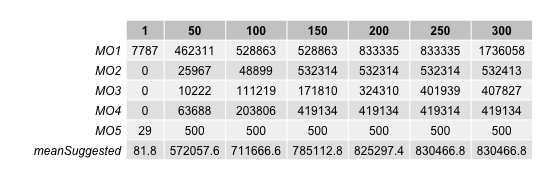
\includegraphics[scale=0.7,center]{compare.png}
% \caption{Rows cleared every 50 iterations}
% \label{fig:compareParameters}
% \end{figure}

From Table \ref{tab:compareParameters}, it is clear that the PSO run using \emph{MO1}'s parameters performed the best, while other MO parameters did not perform as well. In particular, the PSO run using \emph{MO1} managed to clear 1.7 million rows, approximately twice that of \emph{meanSuggested}.

Hence, it is clear that \emph{MO1} parameters are distinctly better for finding the optimal weights for PSO. It is further suggested that for this particular problem, the \emph{MO1} parameters can be refined by running the LUS algorithm starting with \emph{MO1}'s set of parameters, thus likely achieving a higher score.

\section{Scaling PSO For Big Data: Multi-threading}
% As PSO relies on discrete and encapsulated objects (particles), it is feasible to efficiently scale the algorithm for Big Data via parallelization.
Multi-threading was implemented for each particle via the \emph{Java Callable} class and each thread was run concurrently. This made it possible to run the algorithm on the NUS SoC Compute Cluster, which contains 2x8 physical cores at max frequency of 3.00 GHz. Table \ref{tab:parallel-comparison} shows the difference when the algorithm was run iteratively (no multi-threading) compared to when multi-threading was implemented.

\begin{table}[H]
\small
\centering
\caption{Time comparison}
\label{tab:parallel-comparison}
\begin{tabular}{|l|c|}
\hline
                                      & \textbf{Time for 20 iterations (in seconds)} \\ \hline
\textbf{No multithreading}            & 15364.734                                              \\ \hline
\textbf{Multithreading each Particle} & 3308.58\\ \hline
\end{tabular}
\end{table}
Both versions were run on the same node as two separate tasks on the Compute Cluster. From the result, the multi-threaded version of the algorithm performed \textbf{4.64x} faster than its single-threaded counterpart, demonstrating the effectiveness of parallelization to speed up the application.

\section{Training Results}\label{sec:weights}
After 1000 iterations of training as described in Sections \ref{sec:PSO} and \ref{sec:meta-opt}, the weights obtained were:

% \begin{table}[H]
% \small
% \centering
% \caption{Weights of features $f_i \in Features$}
% \label{my-label}
% \begin{tabular}{|l|l|}
% \hline
% \textbf{MaxHeightIncrease}		& 7887 \\ \hline
% \textbf{RowsCleared}           	& 0    \\ \hline
% \textbf{AvgHeightIncrease}		& 0    \\ \hline
% \textbf{NumHoles}				& 0    \\ \hline
% \textbf{ColumnTransition}       & 29   \\ \hline
% \textbf{AbsoluteDiff} 			& 81.8 \\ \hline
% \textbf{RowTransition}          &      \\ \hline
% \textbf{WellSum}				&      \\ \hline
% \end{tabular}
% \end{table}

$$
\left( \begin{array}{c} 
MaxHeightIncrease
\\RowsCleared
\\AvgHeightIncrease
\\NumHoles
\\ColumnTransition
\\AbsoluteDiff
\\RowTransition
\\WellSum
\end{array} \right)
\Longleftarrow\left( \begin{array}{c}
-5.194814083947793
\\5.53478180043909,
\\-2.1920993360428604
\\-5.9838083427614395
\\-12.880189747449215
\\-1.3227027198368309
\\-3.7823922425956837
\\-2.2176395274310137
\end{array} \right)
$$

% * <matilds@live.se> 2018-04-17T14:51:38.948Z:
% 
% less height/smaller height ?? what word to use
% 
% ^ <matilds@live.se> 2018-04-19T04:55:29.200Z.

\section{Results}
The results of 100 runs using the weights obtained in Section \ref{sec:weights} can be seen in Fig. \ref{fig:results}, and the statistical findings in Table \ref{tab:results}.

\begin{figure}[H]
    \centering
    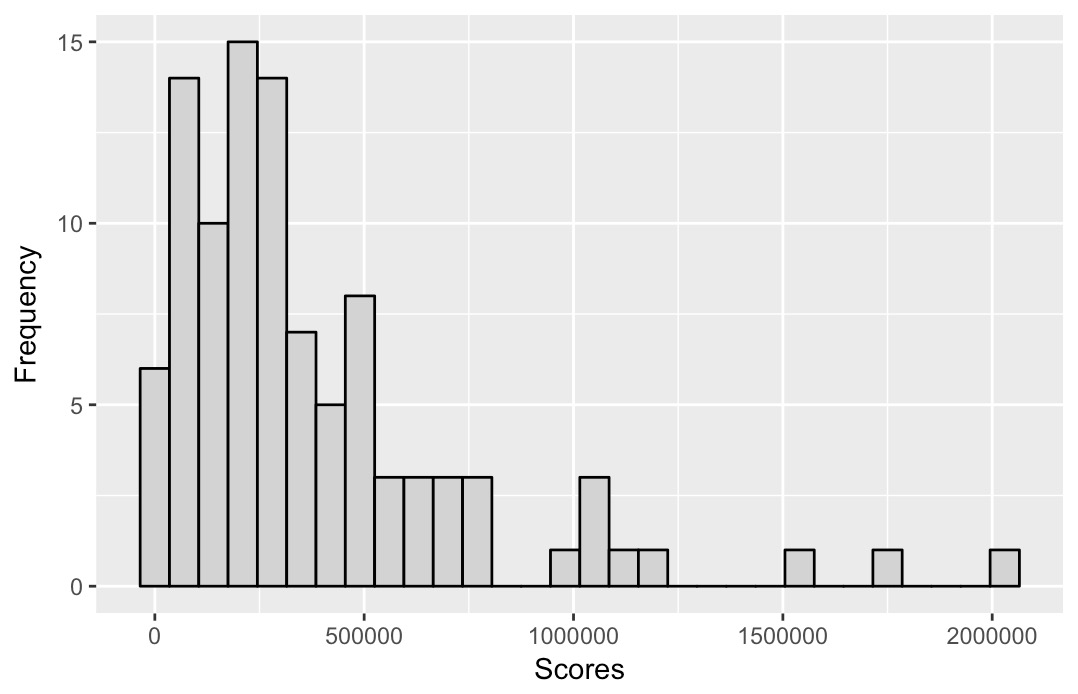
\includegraphics[scale=0.3]{results-frequency-graph.jpeg}
    \caption{Graph of the results of 100 runs}
    \label{fig:results}
\end{figure}

\begin{table}[H]
\small
\centering
\caption{Statistics of 100 runs}
  \label{tab:results}
\begin{tabular}{|c|c|c|c|c|c|}
\hline
{\textbf{Games Played}} & {\textbf{Mean}} & {\textbf{Median}} & {\textbf{Std. Dev.}} & {\textbf{Min}} & {\textbf{Max}} 	\\ \hline
100 & 375,299.22 & 287,109.5 & 366,742.303 & 6,667 & \textbf{2,042,624}		\\ \hline
\end{tabular}
\end{table}


As seen in Figure \ref{fig:results}, there is a significant leftwards skewness of the scores, where on average the agent clears 375k lines, and its best cleared 2 million lines. There is also a significantly large standard deviation of 367k, meaning that the agent's performance is highly variable.

\section{Conclusion}
In conclusion, Particle Swarm Optimization is a good algorithm to apply to this problem, given that it converges to a relatively good position in a small number of iterations. 

A successful parallelization was employed during the training process, with each particle being played in a separate thread, achieving a speedup of 4.64x.

However, a bad feature of PSO is that it may be stuck in a local maxima relatively quickly if the parameters $\omega, \phi_p, \phi_g$ and \emph{swarm size} were set too low or too aggressively. With this in mind, Meta Optimization was applied to find better parameter values, which were employed to hopefully get better positions for the particles $\vec{x}$.  In the end a high score of \textbf{2,042,624} was achieved (from the old high score of 1,414,172 before parameters were tuned).

In addition, it is also important to note that this high score is not very high - others have managed to reach scores of more than 10 million \cite{ThieryImprovementsCROSS-ENTROPY}. This may be becausethe implementation is missing out on some crucial features or the implementation of PSO may have caused the agent to be stuck in a local maxima.
 
\newpage
\appendix
\section{Appendix}
\subsection{Particle Swarm Optimization (PSO) algorithm}\label{app:pso}
For each particle $\vec{x}_i$ for $i=1...N$, where $N$ is the number of particles in the swarm, 

Initialize $\vec{x_i}$'s position $\vec{p}$ with a uniformly distributed random vector: $\vec{x_i} \sim U(\vec{b_{lo}}, \vec{b_{up}})$

Initialize the particle's best known position \emph{pBest} to its initial position: $pBest \leftarrow \vec{x_i}$

If $\emph{globalBest} > \emph{pBest}$, update swarm's best positions $\vec{g} \leftarrow \vec{p_i}$

\noindent While termination criterion not met (for this case number of iterations),

Play game with particle's position $\vec{p_i}$, obtain score $s_i$

If $s_i > pBest$ update: $pBest \leftarrow s_i, \vec{p_i} \leftarrow \vec{x_i}$

If $s_i > gBest$ update: $gBest \leftarrow s_i, \vec{g} \leftarrow \vec{p_i}$

Update $\vec{x_i}$\\

\noindent The movement of each particle $\vec{x}_i$ is guided by the formulae
\begin{gather*}
\vec{v}\leftarrow \omega\vec{v} + \phi_p r_p ( \vec{p} - \vec{x} ) + \phi_g r_g ( \vec{g} - \vec{x} )
\\
\vec{x}\leftarrow \vec{x} + \vec{v}
\end{gather*}
where $\vec{p}$ is the particle's \emph{personal best position} and $\vec{g}$ is the swarm's \emph{global best position}, $\phi_p$ and $\phi_g$ being the \emph{social} and \emph{cognitive coefficient} respectively, emulating the swarm's willingness to move in the search-space. 

$\phi_p$ acts as the particle's ``memory'', causing it to return to its individual best regions of the search space, while $\phi_g$ guides the particle to move to the localized search-space where the global best position was discovered. $r_p$ and $r_g$ are two random real values $\in\left[0..1\right]$ generated every assignment to $\vec{v}$. 

$\omega$ refers to the \emph{inertia} of the particle, and keeps the particle moving in the same direction it was originally heading. A lower value speeds up convergence of the swarm in the search space, and a higher value encourages exploring the search-space.

The values $b_{lo}$ and $b_{up}$ are respectively the lower and upper boundaries of the search-space. The parameters $\omega, \phi_p$, and $\phi_g$ are selected using the values stated in \cite{VanDenBergh2006ATrajectories} 

\subsection{Local Unimodal Sampling (LUS) algorithm}\label{app:lus}
\begin{itemize}
\item Initialise $\vec{x}$ to a random solution in the search space:
\\
\centerline{$\vec{x} \sim U(\vec{b_{lo}}, \vec{b_{up}})$}
\\
Where $\vec{b_{lo}}$ and $\vec{b_{up}}$ are the search-space boundaries.
\item Set the initial sampling space $\vec{d}$ to cover the entire search-space:
\\
\centerline{$\vec{d} \leftarrow \vec{b_{up}} - \vec{b_{lo}}$}
\item Until a termination criterion is met, repeat the following: 
	\begin{itemize}
	\item Pick a random vector $\vec{a} \sim U(-\vec{d}, \vec{d})$
    \item Add this to the current solution $\vec{x}$, to create the new potential solution $\vec{y}$
    \centerline {$\vec{y} = \vec{x} + \vec{a}$}
    \item If $(f(\vec{y}) < f(\vec{x})$ then update the solution:
    \\
    \centerline{$ \vec{x} \leftarrow \vec{y}$}
    \\
    Otherwise decrease the search-range by multiplication with the factor $q$, defined as $2^{-\beta / n}$, where $\beta$ is arbitrarily defined and $n$ is the number of times the search-range has been reduced.
    \\
    \centerline{$\vec{d} \leftarrow q \cdot \vec{d}$}
    \\
    Note that $f:\R^n \rightarrow \R $ is the maximum number of rows cleared by PSO algorithm using $\vec{x}$.
	\end{itemize}
\end{itemize}

\subsection{Parameters obtained from LUS Algorithm}
\begin{figure}[H]
\centering
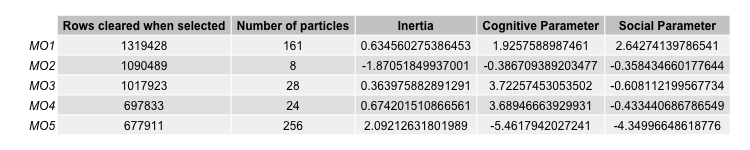
\includegraphics[scale = 0.7]{MOParameters.png}
\caption{Parameters information}
\label{fig:parameters-info}
\end{figure}

\subsection{Various training results}
\begin{figure}[H]
\centering
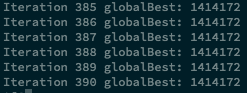
\includegraphics[scale = 1]{1_4mil_score.png}
\caption{Highscore of 1,414,172 before MO}
\end{figure}

\begin{figure}[H]
\centering
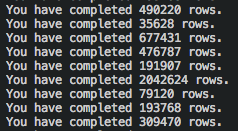
\includegraphics[scale = 1]{2mil_score.png}
\caption{Highscore of 2,042,624 after MO}
\end{figure}

\newpage
\printbibliography

\end{document}





















